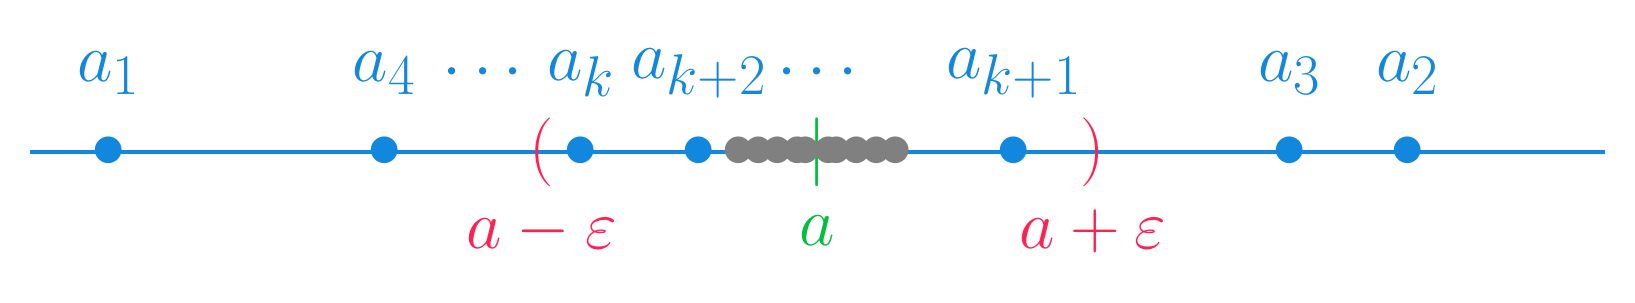
\begin{tikzpicture}[x=5cm,y=5cm]

\Huge
%\newcommand\mydistance{0.1cm}
\definecolor{myblue}{rgb}{0.067,0.529,0.871}
\definecolor{mypurple}{rgb}{0.859,0.071,0.525}
\definecolor{myred}{rgb}{1.0, 0.13, 0.32}
\definecolor{mygreen}{rgb}{0.01, 0.75, 0.24}
\definecolor{mygray}{gray}{0.2}

\draw [ultra thick,myblue] (-2,0) --(2,0);
\draw[mygreen] (0,0) node {$|$};
\draw[mygreen] (0,-0.2) node {$a$};
\draw[myred] (-0.7,0) node {$($};
\draw[myred] (-0.7,-0.2) node {$a-\varepsilon$};
\draw[myred] (0.7,0) node {$)$};
\draw[myred] (0.7,-0.2) node {$a+\varepsilon$};
\draw[myblue] (-1.8,0) node {$\bullet$};
\draw[myblue] (-1.8, 0.2) node {$a_1$};
\draw[myblue] (1.5,0) node {$\bullet$};
\draw[myblue] (1.5, 0.2) node {$a_2$};
\draw[myblue] (1.2,0) node {$\bullet$};
\draw[myblue] (1.2, 0.2) node {$a_3$};
\draw[myblue] (-1.1,0) node {$\bullet$};
\draw[myblue] (-1.1, 0.2) node {$a_4$};
\draw[myblue] (-0.85, 0.2) node {$\cdots$};
\draw[myblue] (-0.6,0) node {$\bullet$};
\draw[myblue] (-0.6, 0.2) node {$a_k$};
\draw[myblue] (0.5,0) node {$\bullet$};
\draw[myblue] (0.5, 0.2) node {$a_{k+1}$};
\draw[myblue] (-0.3,0) node {$\bullet$};
\draw[myblue] (-0.3, 0.2) node {$a_{k+2}$};
\draw[myblue] (0, 0.2) node {$\cdots$};
\draw[gray] (-0.2, 0) node {$\bullet$};
\draw[gray] (-0.15, 0) node {$\bullet$};
\draw[gray] (-0.1, 0) node {$\bullet$};
\draw[gray] (-0.05, 0) node {$\bullet$};
\draw[gray] (-0.03, 0) node {$\bullet$};
\draw[gray] (0.2, 0) node {$\bullet$};
\draw[gray] (0.15, 0) node {$\bullet$};
\draw[gray] (0.1, 0) node {$\bullet$};
\draw[gray] (0.05, 0) node {$\bullet$};
\draw[gray] (0.03, 0) node {$\bullet$};
\end{tikzpicture}